\subsection*{Python Flask}

\subsection*{Implementation}
\subsubsection*{Backend service code}
\begin{lstlisting}[style=Python]
import base64
import label_image
import time

app = Flask(_name_)

@app.route('/classifyImage/', methods=['POST'])
def classify():
    imgdata = base64.b64decode(request.form.get('image'))
    filename = 'images/' + str(time.strftime("%Y%m%d-%H%M%S")) + '.jpg'
    with open(filename, 'wb') as f:
        f.write(imgdata)

    results = label_image.runModel(filename)
    predictions = results[0]

    result_String = ""
    for i in predictions :
        result_String += str(i) + ","
    return result_String

if _name_ == '_main_':
    app.run(host='0.0.0.0', threaded=True)
\end{lstlisting}

\subsubsection*{Method called from 'label\_image.py'}
\begin{lstlisting}[style=Python]
def runModel(file_name):
  model_file = \
    "models/output_graph13.pb"
  label_file = "labels/output_labels13.txt"
  input_height = 299
  input_width = 299
  input_mean = 128
  input_std = 128
  input_layer = "Mul"
  output_layer = "final_result"

  graph = load_graph(model_file)
  t = read_tensor_from_image_file(file_name,
                                  input_height=input_height,
                                  input_width=input_width,
                                  input_mean=input_mean,
                                  input_std=input_std)

  input_name = "import/" + input_layer
  output_name = "import/" + output_layer
  input_operation = graph.get_operation_by_name(input_name)
  output_operation = graph.get_operation_by_name(output_name)

  with tf.Session(graph=graph) as sess:
    results = sess.run(output_operation.outputs[0],
                      {input_operation.outputs[0]: t})
  results = np.squeeze(results)

  top_k = results.argsort()[-5:][::-1]
  labels = load_labels(label_file)

  setIndex = False

  top5_results = [None] * 5
  index = 0
  for i in top_k:
    top5_results[index] = labels[i]
    index += 1

  final_results = [top5_results, results]
  return final_results
\end{lstlisting}

\subsection*{Deployment}
In order to deploy the Flask application to an AWS EC2 instance the following steps had to be followed:

\begin{itemize}
    \item{Upload the output\_graph.pb file (Tensorflow model), the output\_labels.txt file and the source code to the server using SFTP}
    \item{SSH into the server}
    \item{Create a folder called 'images' in the home directory to store uploads images}
    \item{Place model and label files into folders called 'models' and 'labels' respectively}
    \item{Ensure Tensorflow, NOHUP (Ignores the hangup signal in Linux) Python and Flask are installed on the server}
    \item{Ensure no processes are running on port 5000 using the command 'lsof -i :5000'}
    \item{Run the server.py code using the command 'nohup python server.py \&'}
\end{itemize}

\subsubsection*{AWS Architecture}
The application interfaces with an Amazon Web Services (AWS) server called an EC2 instance.
In order to keep the application secure AWS was used to provide a secure architecture.
A Virtual Private Cloud (VPC) was created to host the instances.
In a production environment a load balancer could be used to evenly distribute traffic across a fleet of backend instances but for the purposes of this prototype application, a single instance as in Figure \ref{fig:aws} could be used.
In Figure \ref{fig:aws} the instance is located inside a subnet which is in turn loocated in a VPC.
The purpose of a VPC is to have a virtual network dedicated to a users individual account. 
\begin{figure}[h]
    \centering
    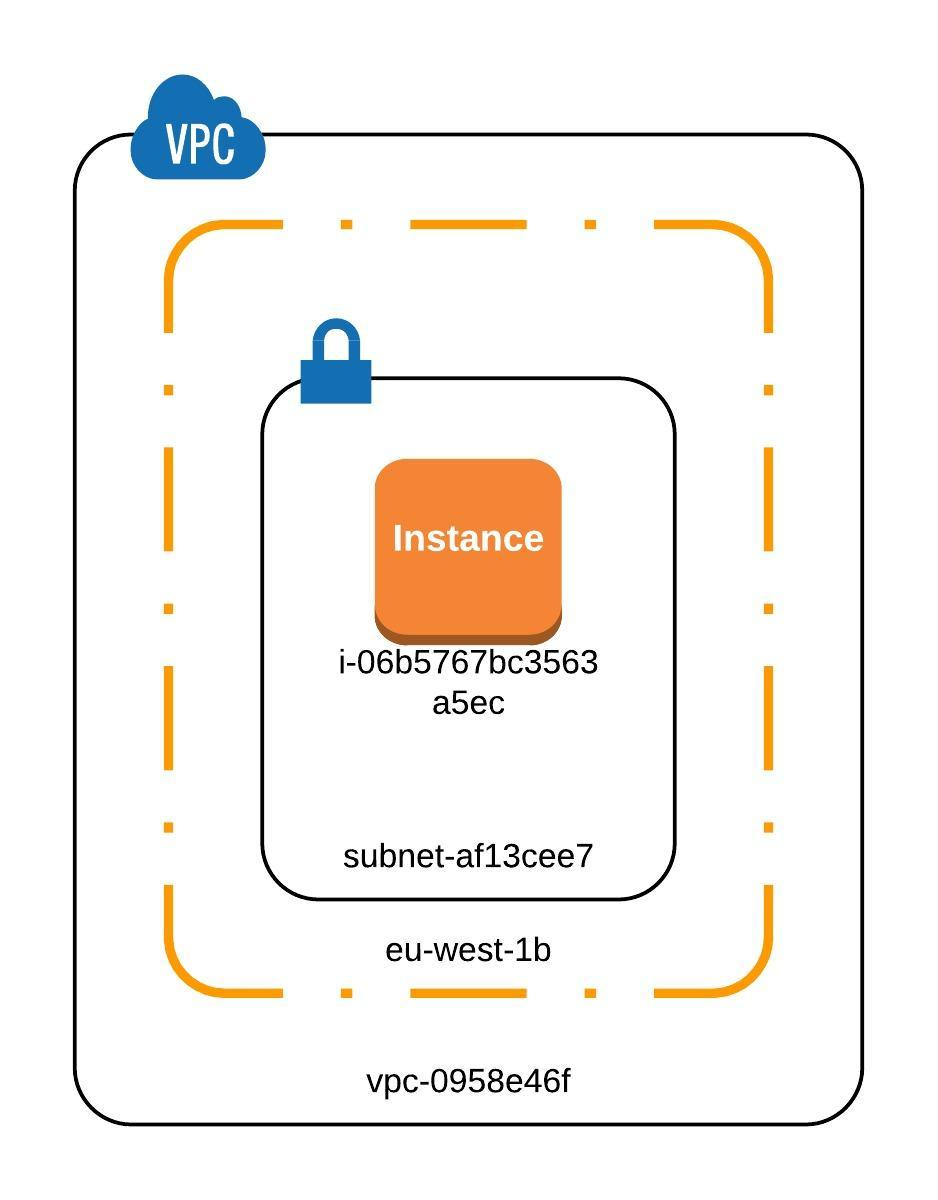
\includegraphics{aws}
    \caption{AWS Network Diagram}
    \label{fig:aws}
\end{figure}

Security groups were utilised to restrict the type of traffic that would be allowed to reach the instance, so that the instance would only receive http requests at port 5000 and receive ssh connections at port 22 as per Figure \ref{fig:awsSecGroup}.
\begin{figure}[h]
    \centering
    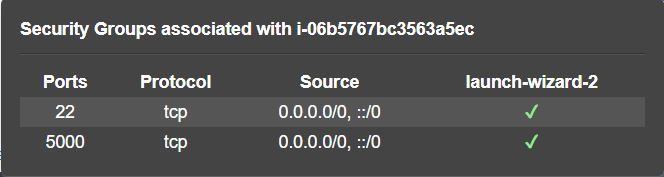
\includegraphics{secGroups}
    \caption{AWS Security Group}
    \label{fig:awsSecGroup}
\end{figure}

% \begin{itemize}
%     \item{Upload the output_graph.pb file (Tensorflow model), the output_labels.txt file and the source code to the server using SFTP}
%     \item{SSH into the server}
%     \item{Create a folder called 'images' in the home directory to store uploads images}
%     \item{Place model and label files into folders called 'models' and 'labels' respectively}
%     \item{Ensure Tensorflow, NOHUP (Ignores the hangup signal in Linux) Python and Flask are installed on the server}
%     \item{Ensure no processes are running on port 5000 using the command 'lsof -i :5000'}
%     \item{Run the server.py code using the command 'nohup python server.py &'}
% \end{itemize}